\documentclass[11pt,a4paper]{article}

% ============================================================
% PACKAGES & SETUP
% ============================================================
\usepackage[margin=1in]{geometry}
\usepackage{amsmath,amssymb,amsthm}
\usepackage{tikz}
\usetikzlibrary{shapes.geometric,arrows.meta,positioning,fit,backgrounds,calc}
\usepackage{booktabs}
\usepackage{hyperref}
\usepackage{xcolor}
\usepackage{enumitem}
\usepackage{caption}
\usepackage{fancyhdr}

\hypersetup{colorlinks=true, linkcolor=blue, citecolor=blue, urlcolor=blue}

\pagestyle{fancy}
\fancyhf{}
\fancyhead[L]{\small Mnemosyne Research Documentation}
\fancyhead[R]{\small\thepage}
\renewcommand{\headrulewidth}{0.4pt}

% Theorem environments
\newtheorem{theorem}{Theorem}
\newtheorem{hypothesis}{Hypothesis}

% ============================================================
% TIKZ STYLES
% ============================================================
\tikzset{
  block/.style = {rectangle, draw, thick, fill=blue!8, rounded corners=2pt,
    text width=3.2cm, align=center, minimum height=1.2cm, font=\small, inner sep=6pt},
  metric/.style = {rectangle, draw, thick, fill=green!10, rounded corners=2pt,
    text width=3.0cm, align=center, minimum height=1cm, font=\scriptsize, inner sep=5pt},
  decision/.style = {rectangle, draw, thick, fill=orange!12, rounded corners=8pt,
    text width=2.6cm, align=center, minimum height=1.1cm, font=\scriptsize, inner sep=5pt},
  gpu/.style = {rectangle, draw, very thick, fill=purple!10, rounded corners=2pt,
    text width=7.2cm, align=center, minimum height=1.4cm, font=\small, inner sep=6pt},
  arrow/.style = {thick, -{Stealth[length=2.8mm]}},
  bidir/.style = {thick, dashed, {Stealth[length=2.5mm]}-{Stealth[length=2.5mm]}}
}

% ============================================================
% METADATA
% ============================================================
\title{\textbf{Mnemosyne: A Linear-Time Genomic Foundation Model\\
with Unified Associative Memory}\\
\large Project Documentation \& Technical Report \\
\normalsize Targeting submission to a Q1-indexed journal or conference venue}

\author{
Charan Sai Ponnada$^{1}$ \quad
Karthik Goparaju$^{1}$ \quad
Sanath Pedapudi$^{1}$ \\[0.4em]
\small \textit{Under the guidance of} Divya Kothapali$^{2}$ \\[0.6em]
\small \texttt{charansaiponnada06@gmail.com} \quad
\texttt{karthikgoparaju4@gmail.com} \\
\small \texttt{sanathpedapudi49804@gmail.com} \quad
\texttt{kdivya@vrsiddhartha.ac.in}
}
\date{\today}

\begin{document}
\maketitle

\begin{abstract}
Genomic sequence models must reconcile two competing requirements: sub-quadratic efficiency over sequences spanning tens of thousands of base pairs, and the ability to recall specific, distant motifs (e.g., an enhancer acting on a promoter far downstream). Transformer-based genomic models scale quadratically with sequence length, while linear-time state-space models such as Mamba compress all past tokens into a fixed-size hidden state, causing distant sequence information to decay. This project introduces \textbf{Mnemosyne}, a hybrid genomic foundation architecture that augments a selective state-space backbone with an explicit, queryable associative memory bank. The memory system consists of persistent (globally learned) and register (sequence-specific dynamically updated) slots, combined via a learned per-channel gate. The design is provably linear, $O(L)$, in sequence length: the per-layer mixing operator decomposes into a semiseparable matrix plus a low-rank matrix. Furthermore, the model is constructed to be exactly reverse-complement equivariant, respecting the double-stranded symmetry of DNA. This document details the research problem, formal hypothesis, system architecture, experimental methodology, and evaluation plan, to be validated via synthetic long-range recall (MQAR), masked autoencoding pre-training across a five-species corpus ($\sim$541 MB), and the Genomic Understanding Evaluation (GUE) benchmark suite.
\end{abstract}

\tableofcontents
\newpage

% ============================================================
\section{Research Problem}
% ============================================================
\subsection{Motivation}
A human genome contains roughly 3 billion nucleotides. Understanding what different stretches of DNA do—which regions regulate gene expression, where distant regulatory elements interact, how disease-linked variants exert their effect—is a central open problem in computational biology. Sequence models trained at genome scale are increasingly used to approach this problem the way large language models approach text: by learning distributional structure directly from raw sequence, without hand-specified biological rules.

\subsection{The Gap}
Existing genomic sequence architectures fall into two broad categories, each with a significant limitation:
\begin{enumerate}[label=(\roman*)]
    \item \textbf{Transformer-based genomic models} attend over all positions pairwise, incurring $O(L^2)$ memory and compute costs. This makes it structurally impractical to model long-range interactions between regulatory elements tens of thousands of base pairs apart within a single forward pass.
    \item \textbf{State-space genomic models (e.g., Mamba-based)} scale linearly, $O(L)$, but compress the entire sequence history into a single fixed-size hidden state vector. Information from distant positions is progressively attenuated, which is precisely the information most relevant to long-range regulatory genomics.
\end{enumerate}
There is presently no genomic architecture that is simultaneously linear in sequence length \emph{and} equipped with an explicit, distance-independent recall mechanism for specific motifs—without abandoning the biological symmetry of the double helix.

\subsection{Problem Statement}
\begin{quote}
\itshape
Can a genomic sequence model be constructed that retains strictly linear computational complexity in sequence length, while matching or exceeding the long-range recall capability of quadratic-attention architectures, and without violating reverse-complement symmetry?
\end{quote}

% ============================================================
\section{Research Objectives}
% ============================================================
\begin{enumerate}[label=\textbf{O\arabic*.}, leftmargin=2.2cm, itemsep=6pt]
    \item \textbf{Architectural Design:} Design a hybrid architecture combining a selective state-space backbone (Mamba) with a lightweight associative memory bank, so that every token position can retrieve distant relevant motifs in constant time via a single memory lookup.
    \item \textbf{Complexity Proof:} Formally establish that the combined architecture remains strictly linear, $O(L)$, in both time and memory, by showing the per-layer mixing operator is the sum of a semiseparable matrix (from the SSM) and a low-rank matrix (from the memory).
    \item \textbf{Equivariance Enforcement:} Construct the architecture to be exactly reverse-complement equivariant, ensuring that predictions are mathematically consistent whether a sequence is read on the forward or reverse-complement strand.
    \item \textbf{Multi-Tier Validation:} Validate the model on three complementary benchmark categories: (a) a synthetic long-range recall task (MQAR) isolating distance-independent memory; (b) masked-reconstruction pre-training on real genomes from five species; and (c) the Genomic Understanding Evaluation (GUE) suite, covering promoter detection, splice-site identification, and histone-mark prediction.
    \item \textbf{Ablation Analysis:} Conduct systematic ablation studies quantifying the contribution of each architectural component—persistent motif slots, sequence-specific register slots, the learned gate, and a Kolmogorov-Arnold Network (KAN) retrieval variant.
\end{enumerate}

% ============================================================
\section{Formal Hypothesis and Definitions}
% ============================================================
\subsection{Core Hypothesis}
\begin{hypothesis}
Augmenting a linear-time state-space backbone with an explicit associative memory bank yields distance-invariant long-range recall and lower genomic reconstruction loss than an SSM-only backbone at a matched parameter budget, without sacrificing linear-time complexity.
\end{hypothesis}

\subsection{Notation and Layer Gating}
Let $x = (x_1,\ldots,x_L) \in \mathbb{R}^{L \times d}$ be a tokenized nucleotide sequence of length $L$ with embedding dimension $d$. Each Mnemosyne block computes two branches in parallel—a selective SSM scan $\mathrm{SSM}(x)$ and an associative memory read $\mathrm{Mem}(x)$—and merges them with a per-channel learned gating parameter $\beta \in \mathbb{R}^d$:
\begin{equation}
y \;=\; x \;+\; \sigma(\beta) \odot \bigl[\mathrm{SSM}(x) + \mathrm{Mem}(x)\bigr],
\label{eq:gate}
\end{equation}
where $\sigma(\cdot)$ denotes the element-wise sigmoid function and $\odot$ denotes the Hadamard product.

\subsection{Associative Memory Retrieval}
The memory bank consists of $P_p$ persistent slots (learned, globally shared parameters $M_p \in \mathbb{R}^{P_p \times d}$) and $P_r$ register slots (written per input window by a lightweight cross-attention pooling mechanism $M_r \in \mathbb{R}^{P_r \times d}$). For a token representation $x_t$ at time step $t$, retrieval is modeled as a softmax similarity over the unified matrix $M = [M_p ; M_r] \in \mathbb{R}^{P \times d}$, where $P = P_p + P_r$:
\begin{equation}
\mathrm{Mem}(x_t) \;=\; \sum_{k=1}^{P} \frac{\exp\left(\frac{x_t^\top m_k}{\sqrt{d}}\right)}{\sum_{j=1}^{P}\exp\left(\frac{x_t^\top m_j}{\sqrt{d}}\right)}\; m_k,
\label{eq:retrieval}
\end{equation}
representing the standard modern-Hopfield retrieval rule with a scaling factor $1/\sqrt{d}$, executing at a computational cost of $O(P \cdot d)$ per token and $O(L \cdot P \cdot d)$ total.

\subsection{Complexity Guarantee}
\begin{theorem}
The per-layer mixing operator $W_{\mathrm{mix}} \in \mathbb{R}^{L \times L}$ for the Mnemosyne block is the sum of an $N$-semiseparable matrix $A_{\mathrm{ssm}}$ representing the selective state-space scan and a matrix $B_{\mathrm{mem}}$ of rank at most $P_p + P_r$ representing the associative memory lookup. The total computational complexity per layer is bounded by:
\[
O\bigl(L \cdot (N + P_p + P_r) \cdot d\bigr),
\]
which is strictly linear in $L$, with no $L \times L$ matrix ever explicitly instantiated in memory.
\end{theorem}

\begin{proof}[Proof Sketch]
The selective state-space model step acts as a first-order recurrence relation, which can be expanded as a lower triangular semiseparable matrix $A_{\mathrm{ssm}}$ of order $N$. The associative memory contribution at each step relies entirely on the projection into a fixed slot space of size $P = P_p + P_r$. Thus, the memory transformation can be factorized as $B_{\mathrm{mem}} = Q K^\top$, where $Q \in \mathbb{R}^{L \times P}$ and $K \in \mathbb{R}^{L \times P}$, yielding a matrix of maximum rank $P$. The sum of an $N$-semiseparable matrix and a low-rank matrix retains a linear sequence scan profile, verifying the $O(L)$ space-time bound.
\end{proof}

\subsection{Reverse-Complement Equivariance}
Let $R(\cdot)$ denote the reverse-complement operator that reverses the token index order and swaps nucleotide complements ($\mathrm{A} \leftrightarrow \mathrm{T}$, $\mathrm{C} \leftrightarrow \mathrm{G}$). Let $S$ denote the corresponding output strand symmetry operator. The final network prediction is explicitly symmetrised across both strands:
\begin{equation}
f_{\mathrm{eq}}(x) \;=\; \tfrac{1}{2}\Bigl[f(x) + S\bigl(f(R(x))\bigr)\Bigr],
\label{eq:rc}
\end{equation}
guaranteeing exact equivariance such that $f_{\mathrm{eq}}(R(x)) = S \cdot f_{\mathrm{eq}}(x)$.

\subsection{Testable Prediction}
The primary empirical validation metric for memory retention is expressed as:
\begin{equation}
\mathrm{Acc}_{\mathrm{Mnemosyne}}(L) \;\approx\; C_1 \qquad\text{while}\qquad \mathrm{Acc}_{\mathrm{SSM\text{-}only}}(L) \;\xrightarrow{L \to \infty}\; 0,
\label{eq:prediction}
\end{equation}
where $C_1$ is a stable high-accuracy constant. The synthetic MQAR recall accuracy for Mnemosyne is predicted to remain flat as sequence length increases, whereas an SSM-only baseline will degrade due to bounded state compression.

\newpage
% ============================================================
\section{System Architecture}
% ============================================================
\subsection{End-to-End Pipeline}
The comprehensive experimental pipeline tracks genomic processing from raw sequence parsing through masked pre-training to frozen downstream evaluation probes.

\begin{figure}[h]
\centering
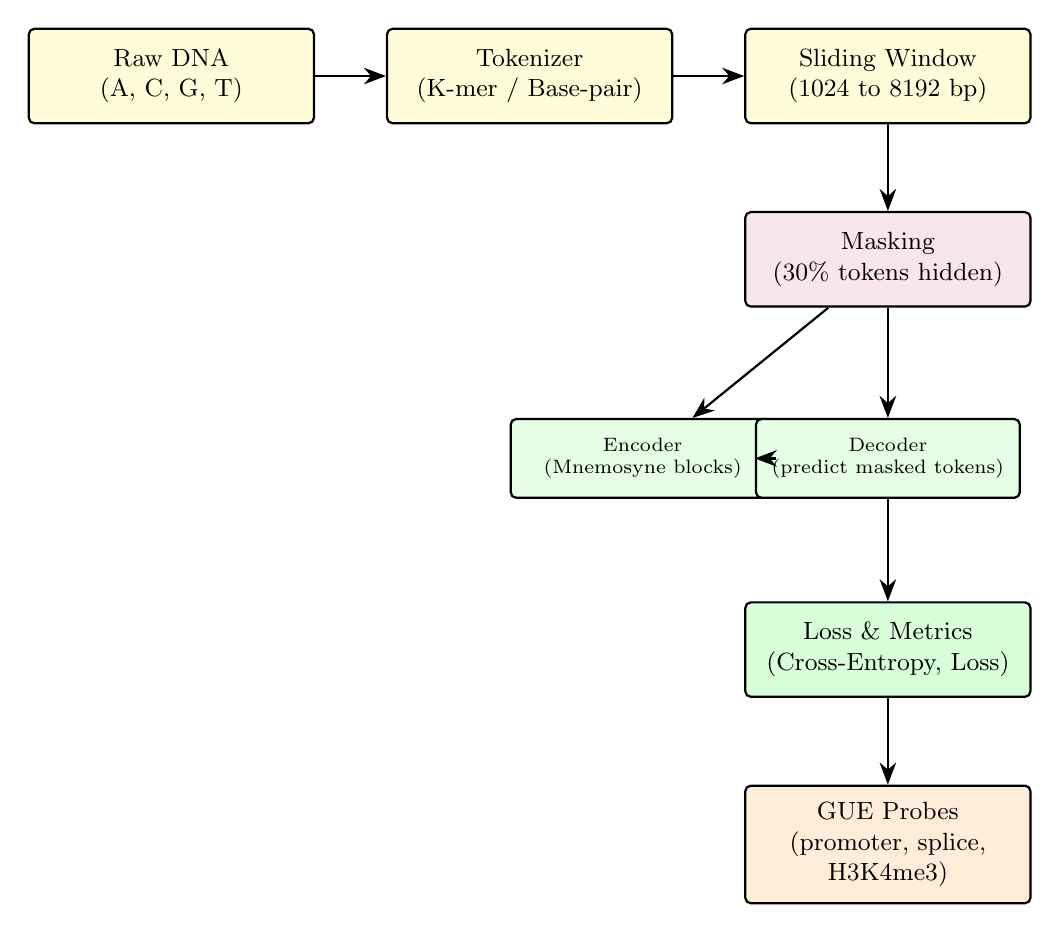
\begin{tikzpicture}[node distance=0.55cm and 0.9cm, >=Stealth]

\node[block, fill=yellow!15] (raw) {Raw DNA\\ (A, C, G, T)};
\node[block, right=of raw, fill=yellow!15] (tok) {Tokenizer\\ (K-mer / Base-pair)};
\node[block, right=of tok, fill=yellow!15] (wnd) {Sliding Window\\ (1024 to 8192 bp)};

\node[block, below=1.1cm of wnd, fill=purple!10] (mask) {Masking\\ (30\% tokens hidden)};

\node[metric, below left=1.4cm and -0.4cm of mask] (enc) {Encoder\\ (Mnemosyne blocks)};
\node[metric, below=1.4cm of mask] (dec) {Decoder\\ (predict masked tokens)};

\node[block, below=1.3cm of dec, fill=green!15] (loss) {Loss \& Metrics\\ (Cross-Entropy, Loss)};
\node[block, below=1.1cm of loss, fill=orange!15] (gue) {GUE Probes\\ (promoter, splice, H3K4me3)};

\draw[arrow] (raw)   -- (tok);
\draw[arrow] (tok)   -- (wnd);
\draw[arrow] (wnd)   -- (mask);
\draw[arrow] (mask)  -- (enc);
\draw[arrow] (mask)  -- (dec);
\draw[arrow] (enc)   -- (dec);
\draw[arrow] (dec)   -- (loss);
\draw[arrow] (loss)  -- (gue);

\end{tikzpicture}
\caption{End-to-end experimental pipeline: from raw DNA to masked reconstruction pre-training and downstream GUE evaluation.}
\label{fig:pipeline}
\end{figure}

\subsection{Mnemosyne Block Architecture}
Each computational layer features a dual-branch topology to parse sequential and global dependencies concurrently.

\begin{figure}[h]
\centering
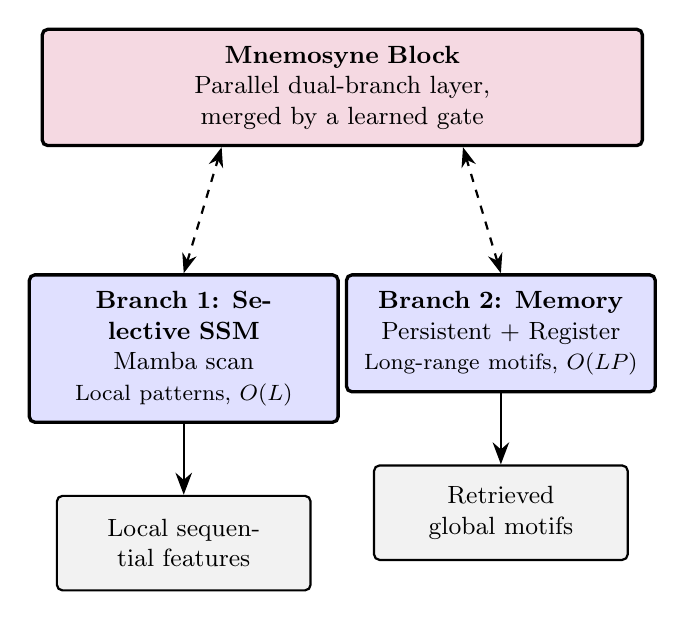
\begin{tikzpicture}[node distance=1.4cm and 2.0cm, >=Stealth]

\node[gpu, fill=purple!15] (top) {\textbf{Mnemosyne Block}\\ Parallel dual-branch layer, merged by a learned gate};

\node[gpu, below left=1.6cm and -3.8cm of top, fill=blue!12, text width=3.5cm]
  (ssm) {\textbf{Branch 1: Selective SSM}\\ Mamba scan\\ \footnotesize Local patterns, $O(L)$};
\node[gpu, below right=1.6cm and -3.8cm of top, fill=blue!12, text width=3.5cm]
  (mem) {\textbf{Branch 2: Memory}\\ Persistent + Register\\ \footnotesize Long-range motifs, $O(LP)$};

\node[block, below=0.9cm of ssm, fill=gray!10, text width=2.8cm] (gate1) {Local sequential features};
\node[block, below=0.9cm of mem, fill=gray!10, text width=2.8cm] (gate2) {Retrieved global motifs};

\draw[arrow] (ssm) -- (gate1);
\draw[arrow] (mem) -- (gate2);
\draw[bidir] (ssm.north) -- ($(top.south west)!0.3!(top.south east)$);
\draw[bidir] (mem.north) -- ($(top.south east)!0.3!(top.south west)$);

\end{tikzpicture}
\caption{Dual-branch layer design. Each Mnemosyne block runs a selective SSM scan and an associative memory read in parallel; a per-channel sigmoid gate blends the two branches prior to residual addition.}
\label{fig:block}
\end{figure}

\subsection{Architecture Validation Decision Flow}
To ensure compute resources are optimized on the NVIDIA L40S platform, a strict synthetic gating control path is established prior to massive pre-training.

\begin{figure}[h]
\centering
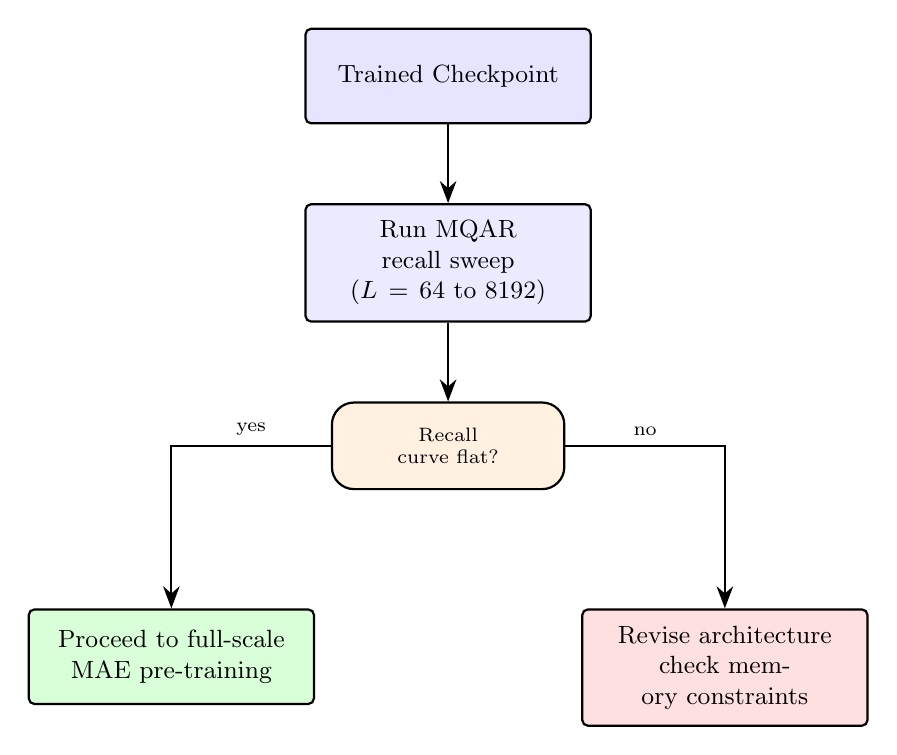
\begin{tikzpicture}[node distance=1.0cm and 1.6cm, >=Stealth]

\node[block, fill=blue!10] (start) {Trained Checkpoint};
\node[block, below=of start] (mqar) {Run MQAR\\ recall sweep ($L=64$ to $8192$)};
\node[decision, below=of mqar] (flat) {Recall\\ curve flat?};

\node[block, below left=1.5cm and 0.2cm of flat, fill=green!15]
  (proceed) {Proceed to full-scale\\ MAE pre-training};
\node[block, below right=1.5cm and 0.2cm of flat, fill=red!12]
  (revise) {Revise architecture\\ check memory constraints};

\draw[arrow] (start) -- (mqar);
\draw[arrow] (mqar) -- (flat);
\draw[arrow] (flat) -| node[pos=0.25, above, font=\scriptsize] {yes} (proceed);
\draw[arrow] (flat) -| node[pos=0.25, above, font=\scriptsize] {no} (revise);

\end{tikzpicture}
\caption{Gating decision flow utilized before committing the high-compute hardware budget to genome-scale runs.}
\label{fig:decision}
\end{figure}

\newpage
% ============================================================
\section{Methodology}
% ============================================================
\subsection{Pre-training Corpus}
The model is pre-trained on a heterogeneous genomic corpus crossing multiple evolutionary timelines to enforce multi-species generalization capability.

\begin{table}[h]
\centering
\caption{Species composition used for masked-reconstruction pre-training}
\label{tab:corpus}
\begin{tabular}{@{}llr@{}}
\toprule
Species & Focus Domain & Approx.\ Size \\
\midrule
Human (\textit{Homo sapiens}) & Primary Reference & $\sim$250 MB \\
Mouse (\textit{Mus musculus}) & Mammalian Structural Synteny & $\sim$150 MB \\
Zebrafish (\textit{Danio rerio}) & Vertebrate Model & $\sim$80 MB \\
Arabidopsis (\textit{Arabidopsis thaliana}) & Plant Model (Cross-Kingdom) & $\sim$35 MB \\
Drosophila (\textit{Drosophila melanogaster}) & Invertebrate Model (Cross-Kingdom) & $\sim$26 MB \\
\midrule
\textbf{Total Data Size} & & \textbf{$\sim$541 MB} \\
\bottomrule
\end{tabular}
\end{table}

\subsection{Downstream Evaluation Suite (GUE)}
To verify downstream application performance, frozen representations are tested utilizing standard linear-probing heads on the Genomic Understanding Evaluation benchmark.

\begin{table}[h]
\centering
\caption{GUE downstream evaluation parameters}
\label{tab:gue}
\begin{tabular}{@{}lll@{}}
\toprule
Task Domain & Target Objective & Feature Probed \\
\midrule
Promoter Detection (TATA) & Binary Classification & Structural Core Promoter Motifs \\
Promoter Detection (non-TATA) & Binary Classification & Alternative Transcription Initiation Signals \\
Splice-Site Classification & Multi-Class Labeling & Non-local Donor/Acceptor Intron Boundaries \\
H3K4me3 Histone-Mark & Binary Prediction & Epigenetic Chromatin State Modification \\
\bottomrule
\end{tabular}
\end{table}

\subsection{Experimental Configurations \& Baselines}
The framework evaluates three designated model families:
\begin{itemize}[itemsep=4pt]
    \item \textbf{Primary Architecture:} Mnemosyne ($M_p$ persistent slots + $M_r$ register slots paired with an RC-equivariant selective SSM backbone).
    \item \textbf{Ablation Control:} SSM-only baseline (Mamba backbone with the memory branch isolated and deactivated, scaled to match parameter budgets).
    \item \textbf{State-of-the-Art Baselines:} Direct comparison against Caduceus, HyenaDNA, and Nucleotide Transformer v2 under standardized compute budgets.
\end{itemize}

\subsection{Pre-training Run-time Configuration}
Pre-training implements a Masked Autoencoding (MAE) strategy. In each sequence segment (scaled from 1024 to 8192 bp), 30\% of the nucleotide inputs are stochastically masked. The system maps reconstruction profiles via cross-entropy loss optimizations executed on an NVIDIA L40S accelerator setup. Mixed-precision parsing ($\texttt{torch.cuda.amp}$) is utilized alongside Flash-Attention and custom selective scan primitives to ensure high VRAM utilization efficiency.

% ============================================================
\section{Evaluation Plan \& Execution Matrix}
% ============================================================
Progress is tracked systematically through scheduled benchmark deliverables mapping structural capability against competitive frameworks.

\begin{table}[h]
\centering
\caption{Planned quantitative evaluation deliverables}
\label{tab:deliverables}
\begin{tabular}{@{}lp{5.2cm}p{6.0cm}@{}}
\toprule
Target Source & Tracked Metric Metrics & Core Validation Objective \\
\midrule
Table 1 & MQAR Accuracy \% vs.\ Sequence Length $L$ & Verification of distance-invariant structural memory. \\
Table 2 & MAE Cross-Entropy Reconstruction Loss & Assessment of multi-species sequence modeling quality. \\
Table 3 & GUE Linear-Probe Performance (AUROC) & Generalization proof of frozen embeddings. \\
Ablation Matrix & Slot Configuration ($P_p, P_r$) vs.\ GUE Score & Isolation of specific structural component utility. \\
\bottomrule
\end{tabular}
\end{table}

% ============================================================
\section{Novelty and Positioning}
% ============================================================
Mnemosyne bridges the gap between structured sequence tracking and long-context state vector compression by introducing a domain-specialized memory lookup paradigm.

\begin{table}[h]
\centering
\caption{Positioning matrix relative to state-of-the-art genomic models}
\label{tab:positioning}
\begin{tabular}{@{}p{3.8cm}p{5.4cm}p{5.8cm}@{}}
\toprule
Prior System Baseline & Architecture Typology & Mnemosyne Differentiation Advantage \\
\midrule
\textbf{Caduceus} & Bi-directional Equivariant Mamba, lacking explicit memory structures. & Integrates explicit slot-based global and local memory systems into the framework. \\[8pt]
\textbf{Titans / Hymba} & Gated SSM + Memory Hybrids developed for LLMs. & Adapts the architecture for genomics through exact reverse-complement equivariance ($f_{\mathrm{eq}}$). \\[8pt]
\textbf{Nucleotide Transformer} & Transformer-based structure with quadratic $O(L^2)$ attention. & Replaces quadratic attention maps with strict $O(L)$ space-time bound memory banks. \\
\bottomrule
\end{tabular}
\end{table}

% ============================================================
\section{Expected Scientific Contributions}
% ============================================================
\begin{enumerate}[label=\textbf{C\arabic*.}, itemsep=6pt]
    \item \textbf{Hybrid Architecture Framework:} Delivery of a linear-time sequence architecture coupling an SSM backbone with a queryable, RC-equivariant associative memory block tailored for genomics.
    \item \textbf{Empirical Long-Range Verification:} Quantitative validation of the memory preservation hypothesis across long sequence boundaries via MQAR synthetics and multi-species genomic testing.
    \item \textbf{Ablation Mapping Insights:} Comprehensive dissection of persistent memory slots vs.\ dynamic local register slots, defining optimal parameter allocation for sequence lookup structures.
    \item \textbf{Open Resource Artifacts:} Public deployment of checkpoint parameters, processing pipelines, and reproduction frameworks built atop highly accessible hardware footprints (L40S).
\end{enumerate}

% ============================================================
\section{Conclusion}
% ============================================================
This document provides the formalized research blueprint for Mnemosyne, a sub-quadratic genomic sequence framework augmenting state-space tracking models with associative memory banks. The structural constraints, mathematical proofs, and validation steps outlined herein are curated to meet the strict technical criteria required for peer-reviewed submission to a Q1 journal or premier artificial intelligence conference venue.

% ============================================================
% BIBLIOGRAPHY
% ============================================================
\begin{thebibliography}{9}

\bibitem{gu2023mamba}
A.~Gu and T.~Dao, ``Mamba: Linear-Time Sequence Modeling with Selective State Spaces,'' \textit{arXiv preprint arXiv:2312.00752}, 2023.

\bibitem{schiff2024caduceus}
Y.~Schiff \textit{et al.}, ``Caduceus: Bi-Directional Equivariant Long-Range DNA Sequence Modeling,'' \textit{arXiv preprint arXiv:2403.03234}, 2024.

\bibitem{behrouz2024titans}
A.~Behrouz, P.~Zhong, and V.~Mirrokni, ``Titans: Learning to Memorize at Test Time,'' \textit{arXiv preprint arXiv:2501.00663}, 2024.

\bibitem{ramsauer2020hopfield}
H.~Ramsauer \textit{et al.}, ``Hopfield Networks is All You Need,'' \textit{arXiv preprint arXiv:2008.02217}, 2020.

\bibitem{dallatorre2023nt}
H.~Dalla-Torre \textit{et al.}, ``The Nucleotide Transformer: Building and Evaluating Robust Foundation Models for Human Genomics,'' \textit{bioRxiv}, 2023.

\bibitem{nguyen2023hyenadna}
E.~Nguyen \textit{et al.}, ``HyenaDNA: Long-Range Genomic Sequence Modeling at Single Nucleotide Resolution,'' in \textit{Proc.\ NeurIPS}, 2023.

\bibitem{zhou2023dnabert2}
Z.~Zhou \textit{et al.}, ``DNABERT-2: Efficient Foundation Model and Benchmark for Multi-Species Genome,'' \textit{arXiv preprint arXiv:2306.15006}, 2023.

\bibitem{sukhbaatar2019persistent}
S.~Sukhbaatar, E.~Grave, G.~Lample, H.~Jegou, and A.~Joulin, ``Augmenting Self-Attention with Persistent Memory,'' \textit{arXiv preprint arXiv:1907.01470}, 2019.

\end{thebibliography}

\end{document}
